\chapter{Pupil Detection}
\label{chap:pupildetection}
\section{Current State}
\label{sec:current}
\subsection{Overview of Algorithm}
The general sequence of the algorithm can be described as follows:
\begin{enumerate}
	\item Find darkest spot
	\item Extract rays  starting from the darkest spot from the image
	\item Transit the rays with a filter of certain length to detect edges
	\item Fit an ellipse on the detected edges with the least square method
\end{enumerate}
The darkest spot is determined by a raster with a fixed distance between points. For each point the average with the surrounding eights point is calculated. The point with the darkest average is the startpoint for the rest of the algorithm.

Outgoing from the startpoint rays are stamped out by the starburst algorithm. This part will run on the FPGA. 

For each ray that is stamped out by the starburst the difference to the next pixel is calculated. Because the edge may not lie on a single pixel surrounding differences are added together to build a score for each pixel. This score is positive for transitions from a darker pixel to a brighter. The pixel with the highest score is determined as detected edge. So only edges that transit from dark to bright can be detected.

Every edgepoint is handed over to a weighted least square method to find a ellipse that fits all the points well.
\subsection{Testing}
The algorithm was tested with pictures that were inserted at compile time with the parameters of the ellipse as output. The result was then compared with the result.
\section{Problem Analysis}
\subsection{Improve Testing}
It is very time consuming to generate picture data that can be compiled and to compare the output of the program with what is expected. A better way would be if a algorithm can read any picture or video file and display the result of the algorithm visually on each picture. 

The program "Gazelle View" that was developed during the project study can already open and play video files. Because of the modular design of Gazelle View it is simple to insert the algorithm during the decode phase and paint the rays, the detected edges and the fitted ellipse on the image.

All data that was produced by the algorithm may also hold important information to find bugs or problems with the algorithm. In order to display that data besides the frame all data is packed into a struct and displayed in a Treeview beside the frame. 

The next step to improve testing would be to automate it and ideally condense the performance of the algorithm to parameters such as the mean and variance of the accuracy.

This should be done on a wide variety of test data, at best with high frame rate pictures that were captured with the eye tracking system. For each of those pictures an ellipse has to be fitted manually and stored as a golden reference. As this needs to be done for a lot of pictures the process of generating the reference needs to be simplified.
\subsection{Outliers}
The supplied algorithm does not differentiate between edges that are from the pupil or other edges from hair or the eyelid. The algorithm works fine when every edge is a right one as seen in figure \ref{fig:oldGood}. But as a consequence to the least square method a single false detection severely alters the fitted ellipse as it happens in figure \ref{fig:oldOutlier}. 
\begin{figure}
	\begin{subfigure}{.5\textwidth}
		\centering
		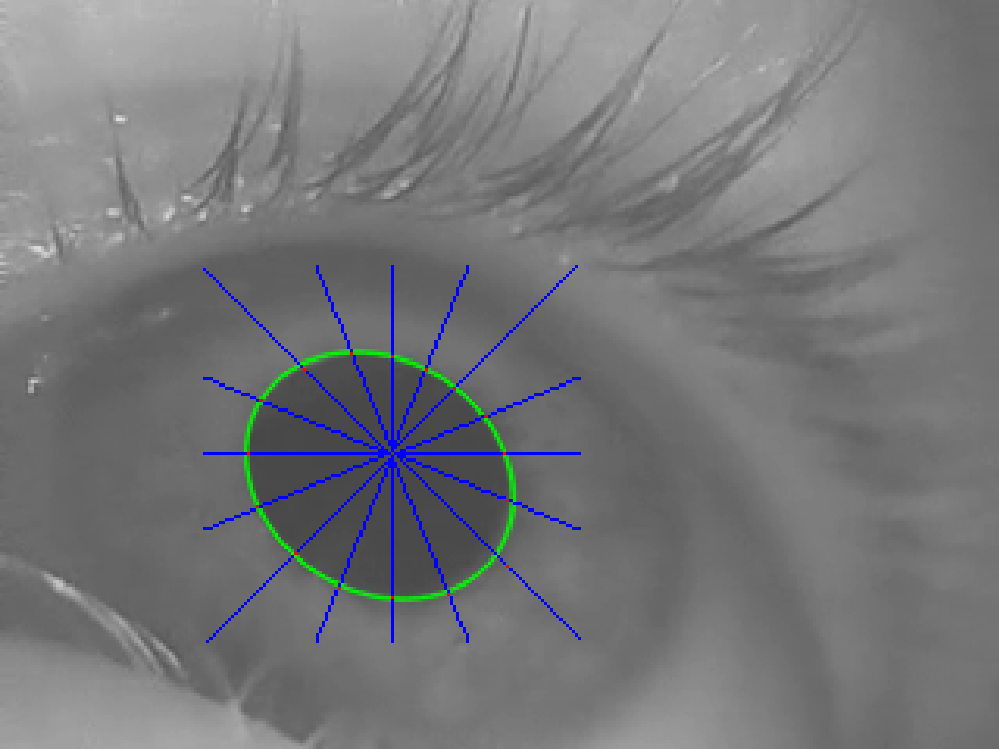
\includegraphics[width=\linewidth]{images/good_fit_old.png}
		\caption{Fitting of Ellipse without outliers}
		\label{fig:oldGood}
	\end{subfigure}%
	\begin{subfigure}{.5\textwidth}
		\centering
		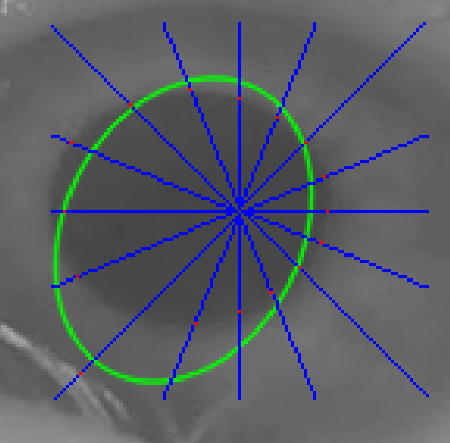
\includegraphics[width=.8\linewidth]{images/outlier_problem.png}
		\caption{Fitting of Ellipse with one outlier}
		\label{fig:oldOutlier}
	\end{subfigure}
\caption{Comparison between results with and without an outlier}

\end{figure}

To mitigate the influence of outlier the occurence needs to be reduced accompanied by the detection of outliers that are still detected.
\section{Algorithm}
\section{Angle-Validation}
\label{sec:angleValidation}
To detect outliers it is necessary to find properties that differ strongly from the other transitions. One of those properties gets visible when the angle for each transition gets calculated with the neighbouring transitions. 

In figure \ref{fig:outlierOutside} a outlier lies on the bottom left corner of the image and outside of the pupil. The angle of the outlier is very small compared to angle of the neighbouring transitions. Those on the other hand have a greater angle than the other transition points. 

When a outlier is inside the pupil then the situation is reversed as visible in figure \ref{fig:outlierInside} where the outlier has a big angle and the adjacent transitions very small angles. 

\begin{figure}[H]
\begin{subfigure}{.33\textwidth}
	\centering
	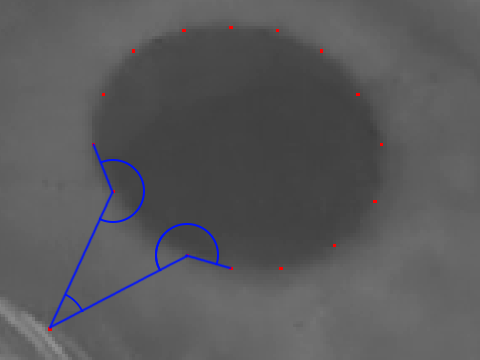
\includegraphics[width=.8\linewidth]{images/angle.png}
	\caption{Outlier outside Pupil}
	\label{fig:outlierOutside}
\end{subfigure}%
\begin{subfigure}{.33\textwidth}
	\centering
	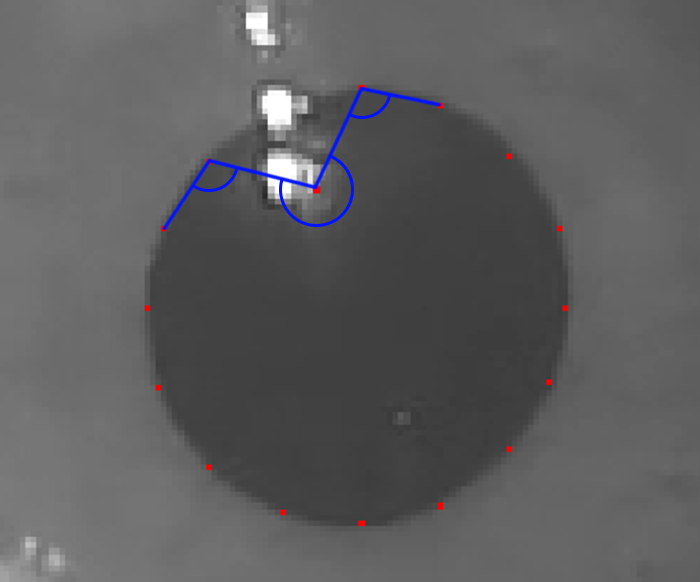
\includegraphics[width=.8\linewidth]{images/outlier_inner.png}
	\caption{Outlier inside Pupil}
	\label{fig:outlierInside}
\end{subfigure}
\begin{subfigure}{.33\textwidth}
	\centering
	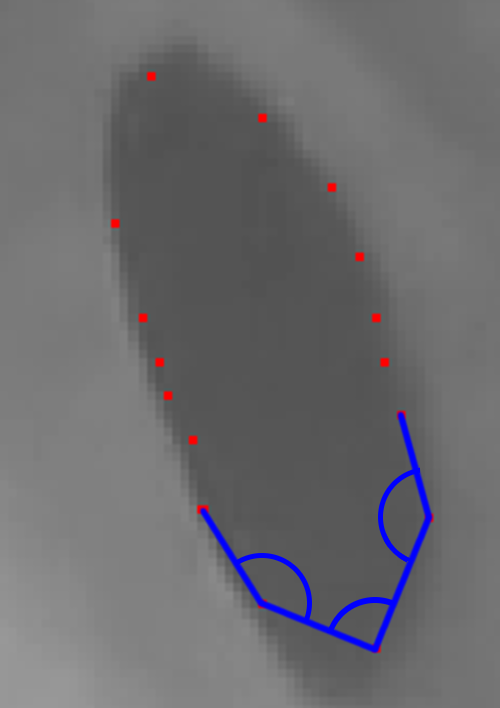
\includegraphics[width=.6\linewidth]{images/non_outlier.png}
	\caption{Accurate Transitions  with small Angles}
	\label{fig:nonOutlier}
\end{subfigure}
\caption{Angles between Transitions around Outliers}
\end{figure}

Multiple adjacent outliers differ in that it is not possible to make a clear statement what the angle will be. But the neighbours to the Outliers still have the same properties as described in the last paragraphs. For that reason an algorithm that wants to detect outliers should focus on detecting the neighbours of outliers.

In figure \ref{fig:nonOutlier} three adjacent transitions have angles that appear too small compared to its neighbours. None of them are outliers.

\subsection{Overview of Algorithm}
\label{sec:descriptionOfAngleValidation}

The algorithm to detect outliers based on the angles between transitions involves four steps:

\begin{enumerate}
	\item Calculate angles
	\item Find 3 adjacent angles with small differences
	\item Categorize angles
	\begin{itemize}
		\item To big
		\item To small
		\item As expected 
	\end{itemize}
	\item Determine outliers
\end{enumerate}
\subsection{Calculate Angles}
\label{sec:calculateAngles}
The angle between the points is calculated with the vectors that stretch from the center point to the other points. For each vector the angle between the x axis and the vector is calculated with the atan2 function. The advantage of the atan2 over the conventional arctangent function is that it takes coordinates and returns the angle for the correct quadrant. The difference of the resulting two angles is the desired angle between the points. 

When the detected transitions are close to each other, measurement uncertainty can greatly affect the angles at such points. To mitigate that effect the angle for a point is only calculated with transitions that are distant enough.
\subsection{Find adjacent angles with small differences}
Context is important to categorize an angle. Only angles that are as expected do not always require context. This is the case when there are three adjacent angles that fall within a narrow range of each other and create context for the neighbouring angles.

\subsection{Categorize Angles}
The found context leads the way to iterate over every transition and categorize the angle within the context. This is done as described in the decision making diagram in \ref{fig:decisionMaking}. Angles are classified into three groups. Angles that are as expected, too big or too small. 

\begin{figure}[H]
	\centering
	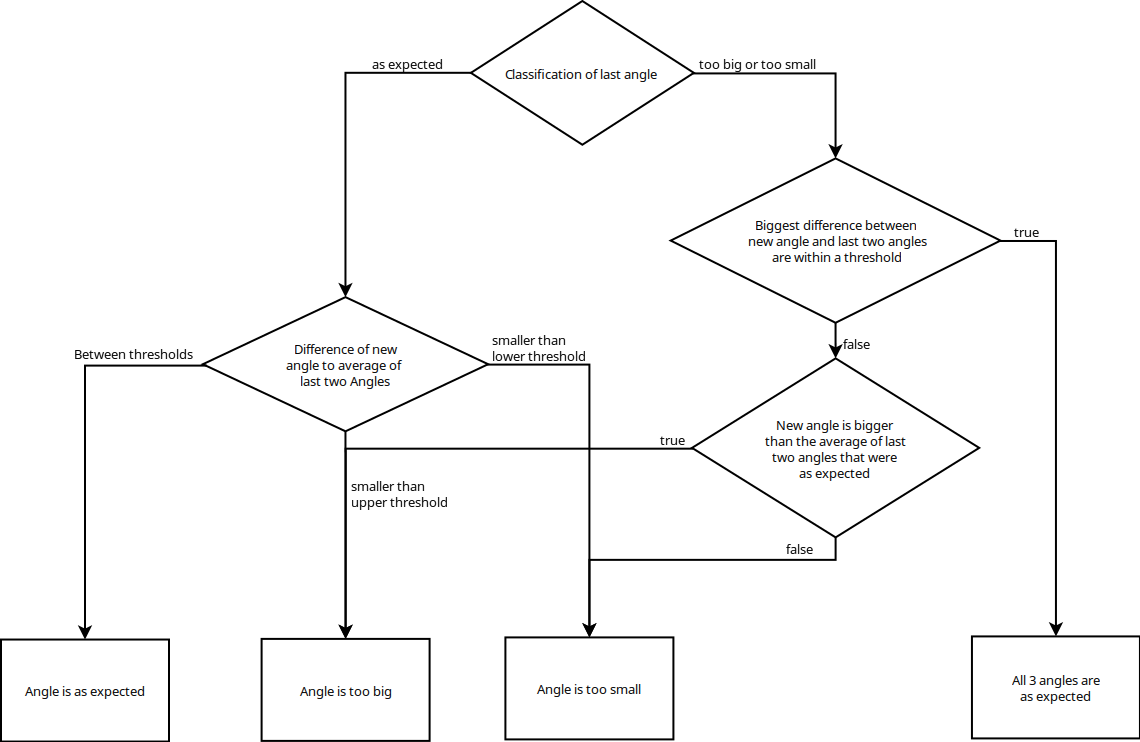
\includegraphics[width=.9\linewidth]{images/angleclassification.png}
	\caption{Decision making diagram for categorizing angles}
	\label{fig:decisionMaking}
\end{figure}
\subsection{Determine outliers}
As described in section \ref{sec:angleValidation} outliers are surrounded by angles that are not as expected. The categorized angles make that determination straight forward. An outlier is a transition where neither the angle before or after is categorized as expected. 
The situation described in figure \ref{fig:nonOutlier} where accurate transitions build three adjacent angles that are smaller than expected constitute an exception to this rule. This exception only occurs with adjacent small angles with neighbours that are as expected. 
\section{Colour of the Startpoint}
\label{sec:colorStartpoint}
The pupil has an uniform colour. So transitions that go from the pupil to the iris start with a colour close to the colour of the startpoint. Transitions from the iris to an eyelid on the other hand start with a colour that is brighter. This correlation can be exploited to improve the number of correctly detected transitions by dividing the score during the filter by the difference to the colour of the startpoint. To avoid a division with zero the absolute difference with an offset is used. Th offset can also be used to control the influence of this part of the algorithm.  
\section{Border Detection}
\label{sec:randdetektion}
The colours of te starburst are represented by the values between one and 255. When a point of the starburst is outside the image it is set to zero. With that it is simple to detect the border during the filter. The behaviour in this case is different depending if there was already a edge or not. If there was already an edge we would like to keep that edge otherwise the result of this ray should be discarded. 

To decide if an edge has already ocured a similar method as in section \ref{sec:colorStartpoint} is used. But instead of adjusting the score of a transitions a hard threshold is applied. 
\section{Exploit good Results}
\label{sec:goodResults}

The high framerate of the eye-capturing cameras results in small differences of the pupil position between frames. This can be used to improve the result because we already have an idea what the ellipse will look like. The startpoint can be adjusted to be the center ofthe old ellipse so the detected edges will be more equally distributed.

With the old ellipse it is also possible to calculate where a ray would transits this ellipse. This information is used to weight the score of a transition similar as the colour of the startpoint in section \label{sec:colorStartpoint} was handled. The score is divided by the absolute distance in pixel to the old ellipse on the ray with a small offset.
\section{Fixed Threshold}
\label{sec:fixedThreshold}
This section is about a method that replaces the ray transition that uses a filter with a threshold. 

An edge is detected when the difference to the colour of the startpoint is greater than a certain threshold. This approach is less flexible than the filter because different light conditions or eyes might require a different threshold. 




